\documentclass{beamer}
\usepackage{caption}
\usepackage{subfigure}
\usetheme[background=light]{metropolis}

\title{\large{Improving Interprocess Communication in Globl/solve \\ \& \\ Improving Slew Models for IVS antennas}}
\date{2016-08-18}
\author{Lina Olandersson, Erik Thorsell, Simon Strandberg}
\institute{Created for NVI Inc. at the Goddard Space Flight Centre}

\begin{document}
    \maketitle

    \begin{frame}{Table of Contents}
    \tableofcontents
    \end{frame}

%%%%%%%%%%%%%%%%%%%%%%%%%%%%%%%%%%%%%%%%%%%%%%%%%%%%%%%%%%%%%%%%%%%%%%%%%%%%%%%

    \section{Learning Fortran}
%%
    \begin{frame}{Server/Client}
        \begin{figure}[ht]
            \centering
            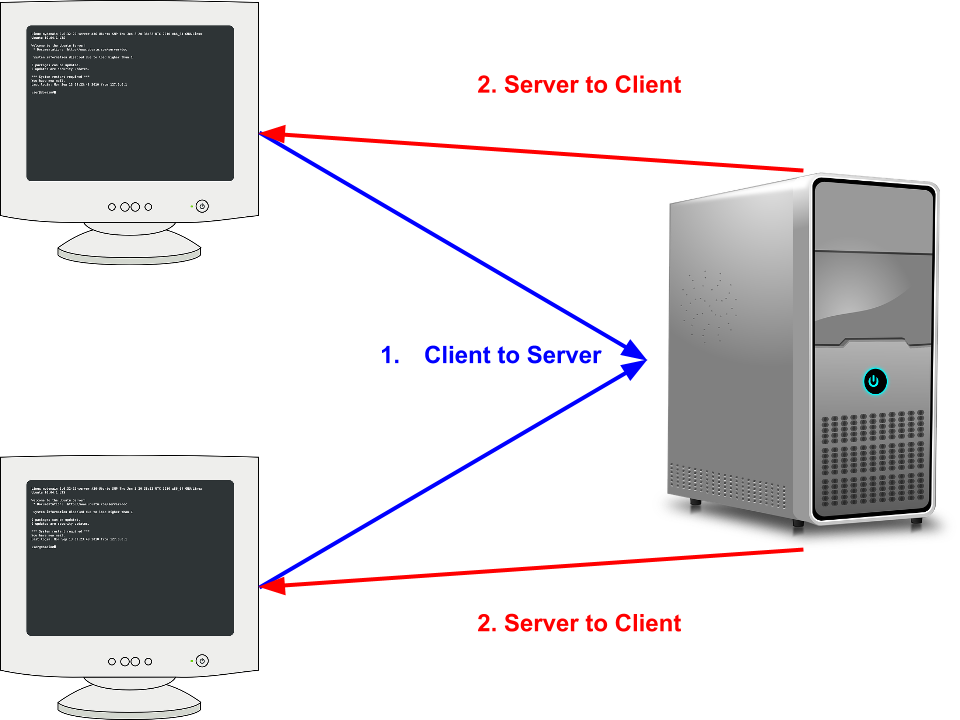
\includegraphics[width=1\columnwidth]{serverclient}
            \caption{A simple server/client structure.}
        \end{figure}
    \end{frame}
%%
    \begin{frame}{Server/Client}
        \begin{figure}[ht]
            \centering
            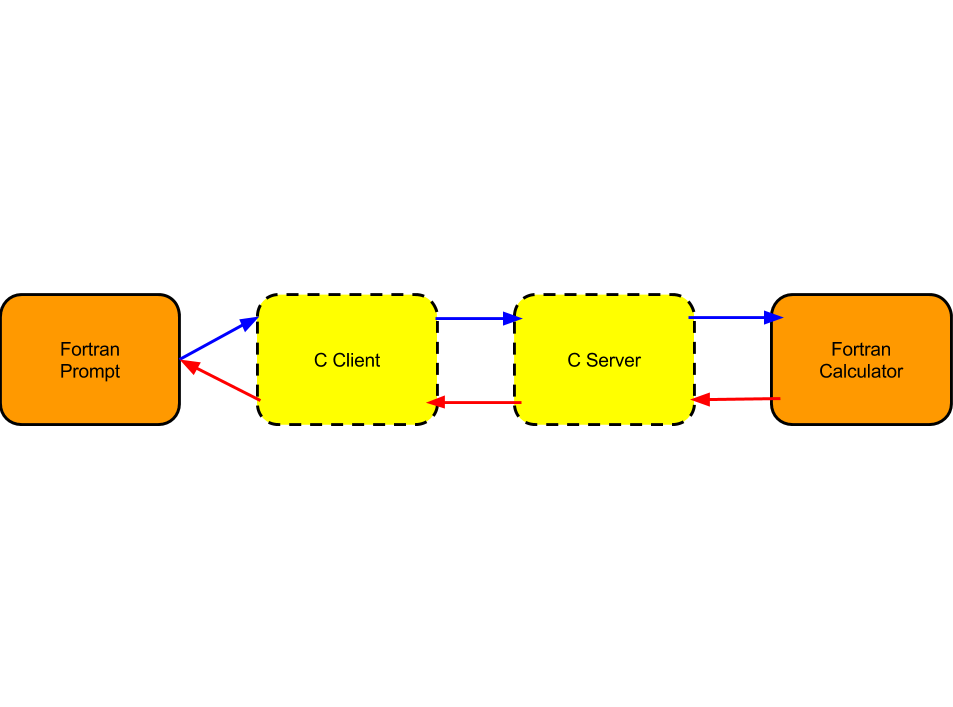
\includegraphics[width=1\columnwidth]{fortrancalculator}
            \caption{How our calculator works.}
        \end{figure}
    \end{frame}
%%
   \begin{frame}{Calculator}
        \begin{figure}[ht]
            \centering
            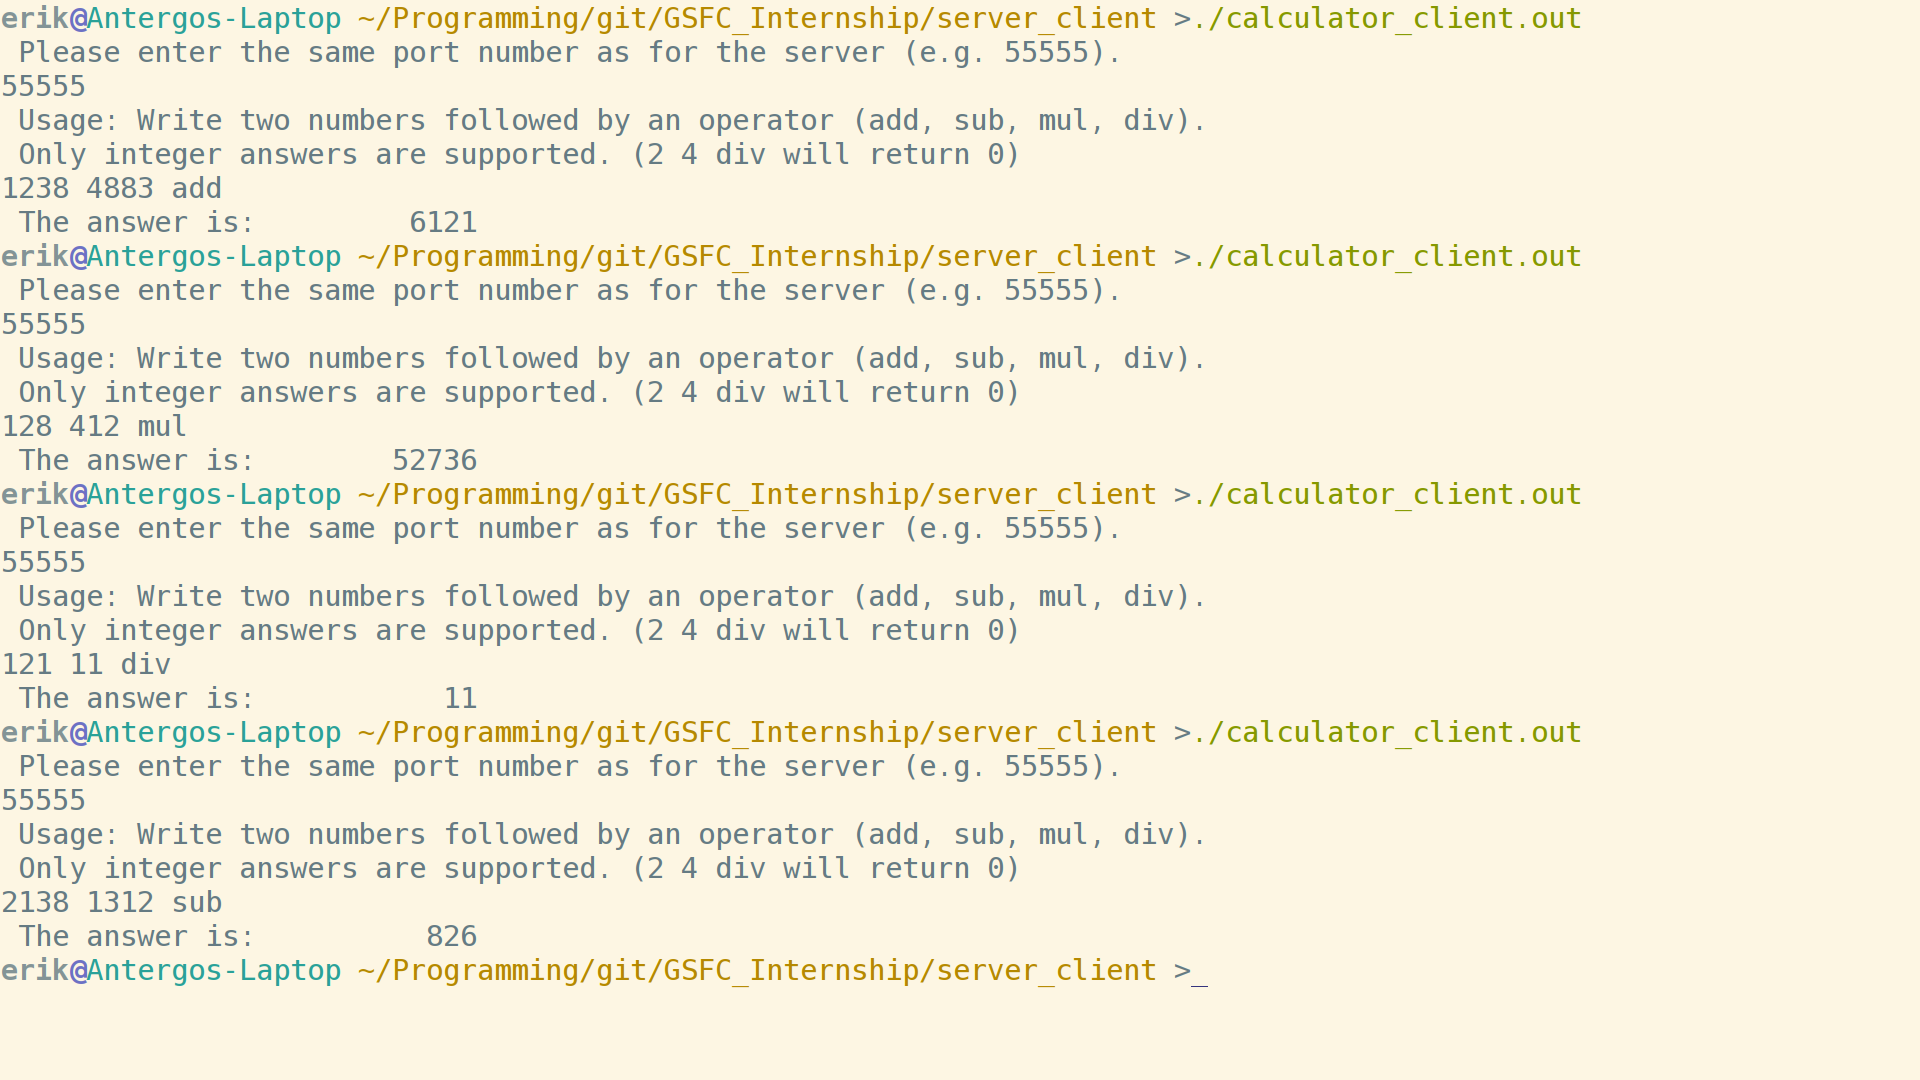
\includegraphics[width=1\columnwidth]{calculator}
            \caption{Example usage of the calculator.}
        \end{figure}
    \end{frame}

%%%%%%%%%%%%%%%%%%%%%%%%%%%%%%%%%%%%%%%%%%%%%%%%%%%%%%%%%%%%%%%%%%%%%%%%%%%%%%%

    \section{Our First Project}

    \begin{frame}{Problem Description}
        Rewrite how Globl/solve handles its passing of data to and from
        userpartials and userprogs.

        By minimizing disc I/O we want to increase the speed at which data is
        sent.
    \end{frame}
%%
    \begin{frame}{Problem Description}
        \begin{figure}[ht]
            \centering
            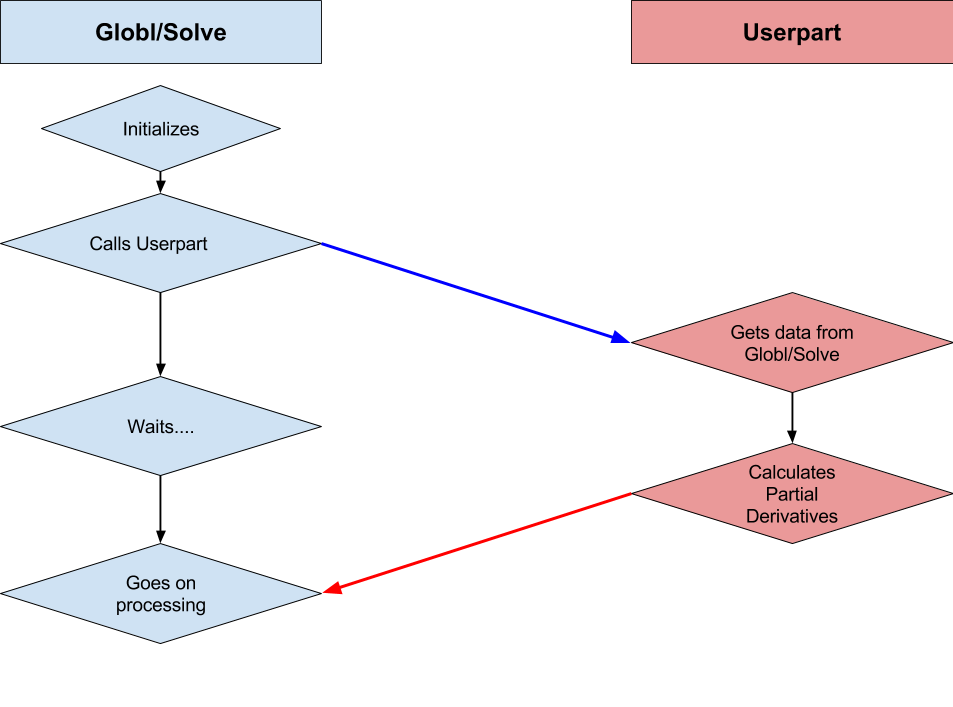
\includegraphics[width=1\columnwidth]{globlsolveblock}
            \caption{Block diagram showing communication between Globl/Solve
                     and Userpart.}
        \end{figure}
    \end{frame}

%%%%%%%%%%%%%%%%%%%%%%%%%%%%%%%%%%%%%%%%%%%%%%%%%%%%%%%%%%%%%%%%%%%%%%%%%%%%%%%
    \section{Testing I/O performance}

    \begin{frame}{I/O Performance}
    Protocols we have tried and used:
    \pause
    \begin{itemize}[<+-|alert@+>]
        \item Using the hard drive:
            \begin{itemize}
                \item Read/Write to \textbf{file}
                \item Sending/Receiving with \textbf{pipes}
            \end{itemize}
        \item Using the memory:
            \begin{itemize}[<+-|alert@+>]
                \item Sending/Receiving with \textbf{TCP/IP} Sockets
                \item Sending/Receiving with \textbf{OpenMPI}
                \item Sending/Receiving with \textbf{ZeroMQ}
            \end{itemize}
    \end{itemize}
    \end{frame}
%%
    \begin{frame}{Performance Test}
        \begin{enumerate}[<+-|alert@+>]
            \item The producer generates a list of length n and fills it with
                  integers.
            \item The producer writes the list to file (or sends it over the
                  designated transfer protocol).
            \item The consumer reads (or receives) the list.
            \item The consumer squares each int in the list and sends it back
                  to the producer.
            \item The producer reads (or receives) the modified list.
        \end{enumerate}
    \end{frame}
%%
    \begin{frame}{Result for I/O Performance}
    \begin{figure}[h!]
        \centering
        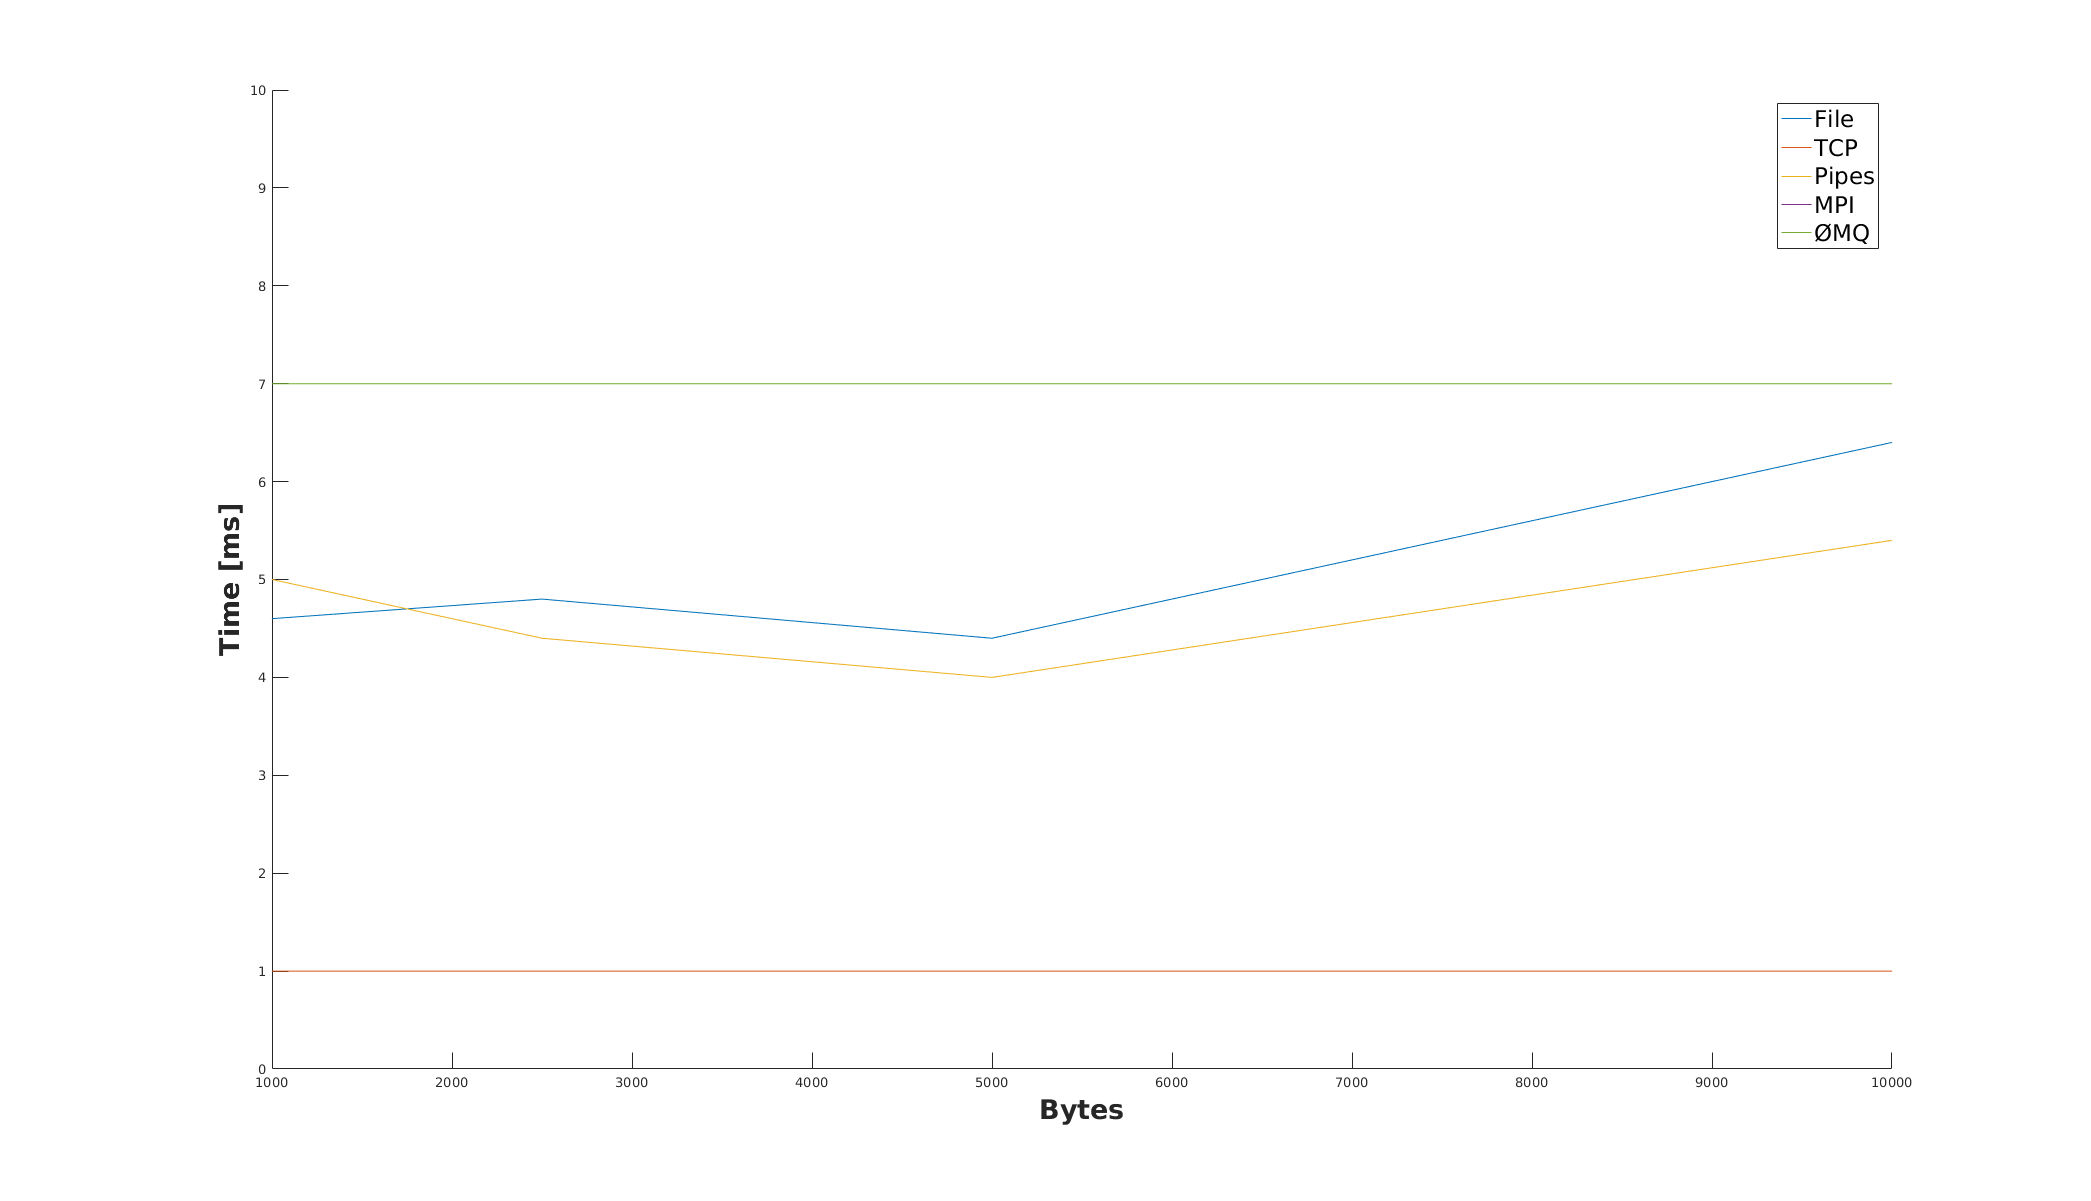
\includegraphics[width=1\columnwidth]{singlerun-nf}
    \end{figure}
    \end{frame}
%%
    \begin{frame}{Result for I/O Performance}
    \begin{figure}[h!]
        \centering
        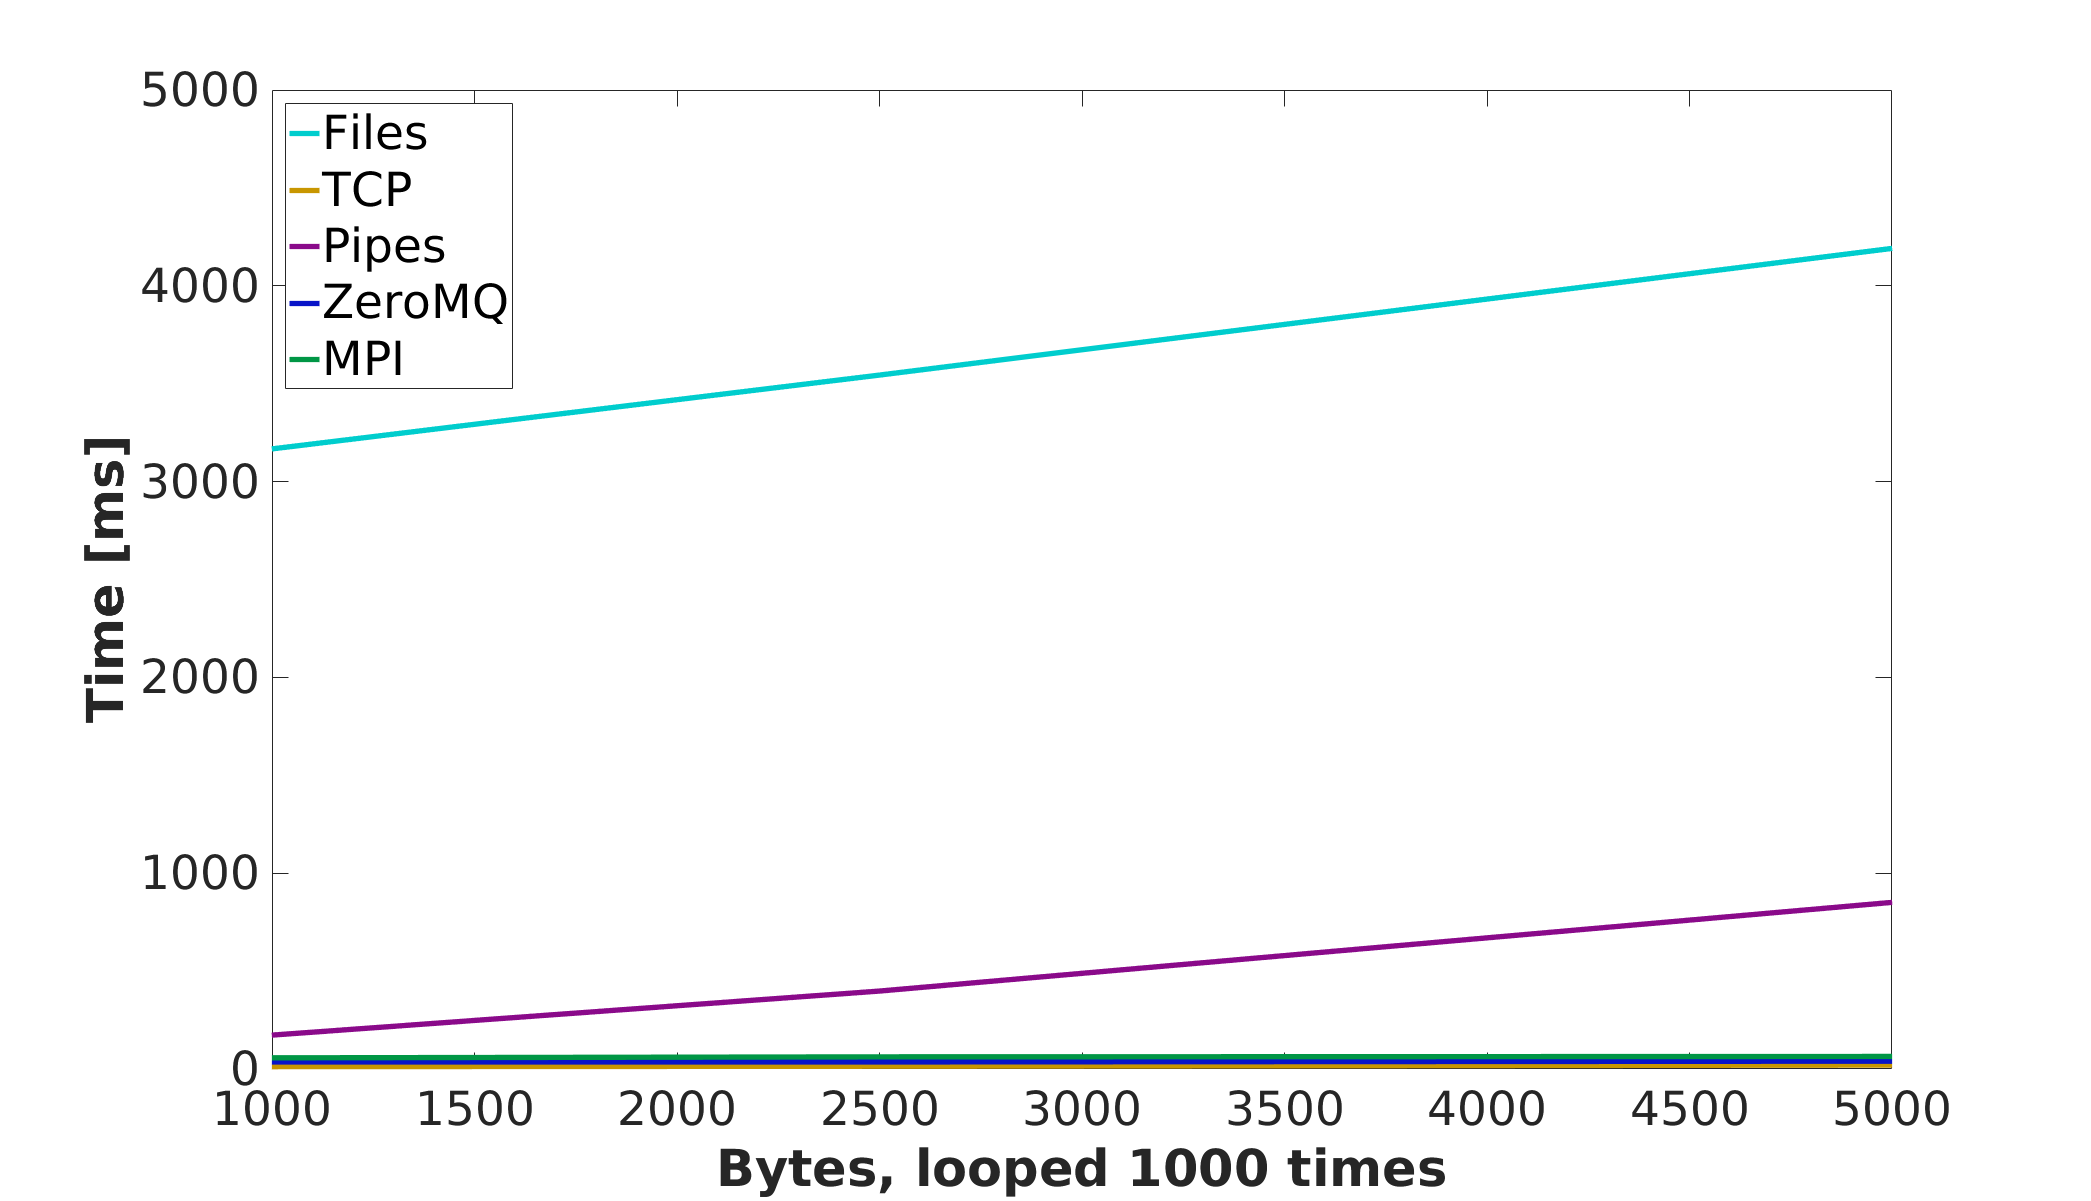
\includegraphics[width=1\columnwidth]{thousandrun+files-nf}
    \end{figure}
    \end{frame}
%%
    \begin{frame}{Result for I/O Performance}
    \begin{figure}[h!]
        \centering
        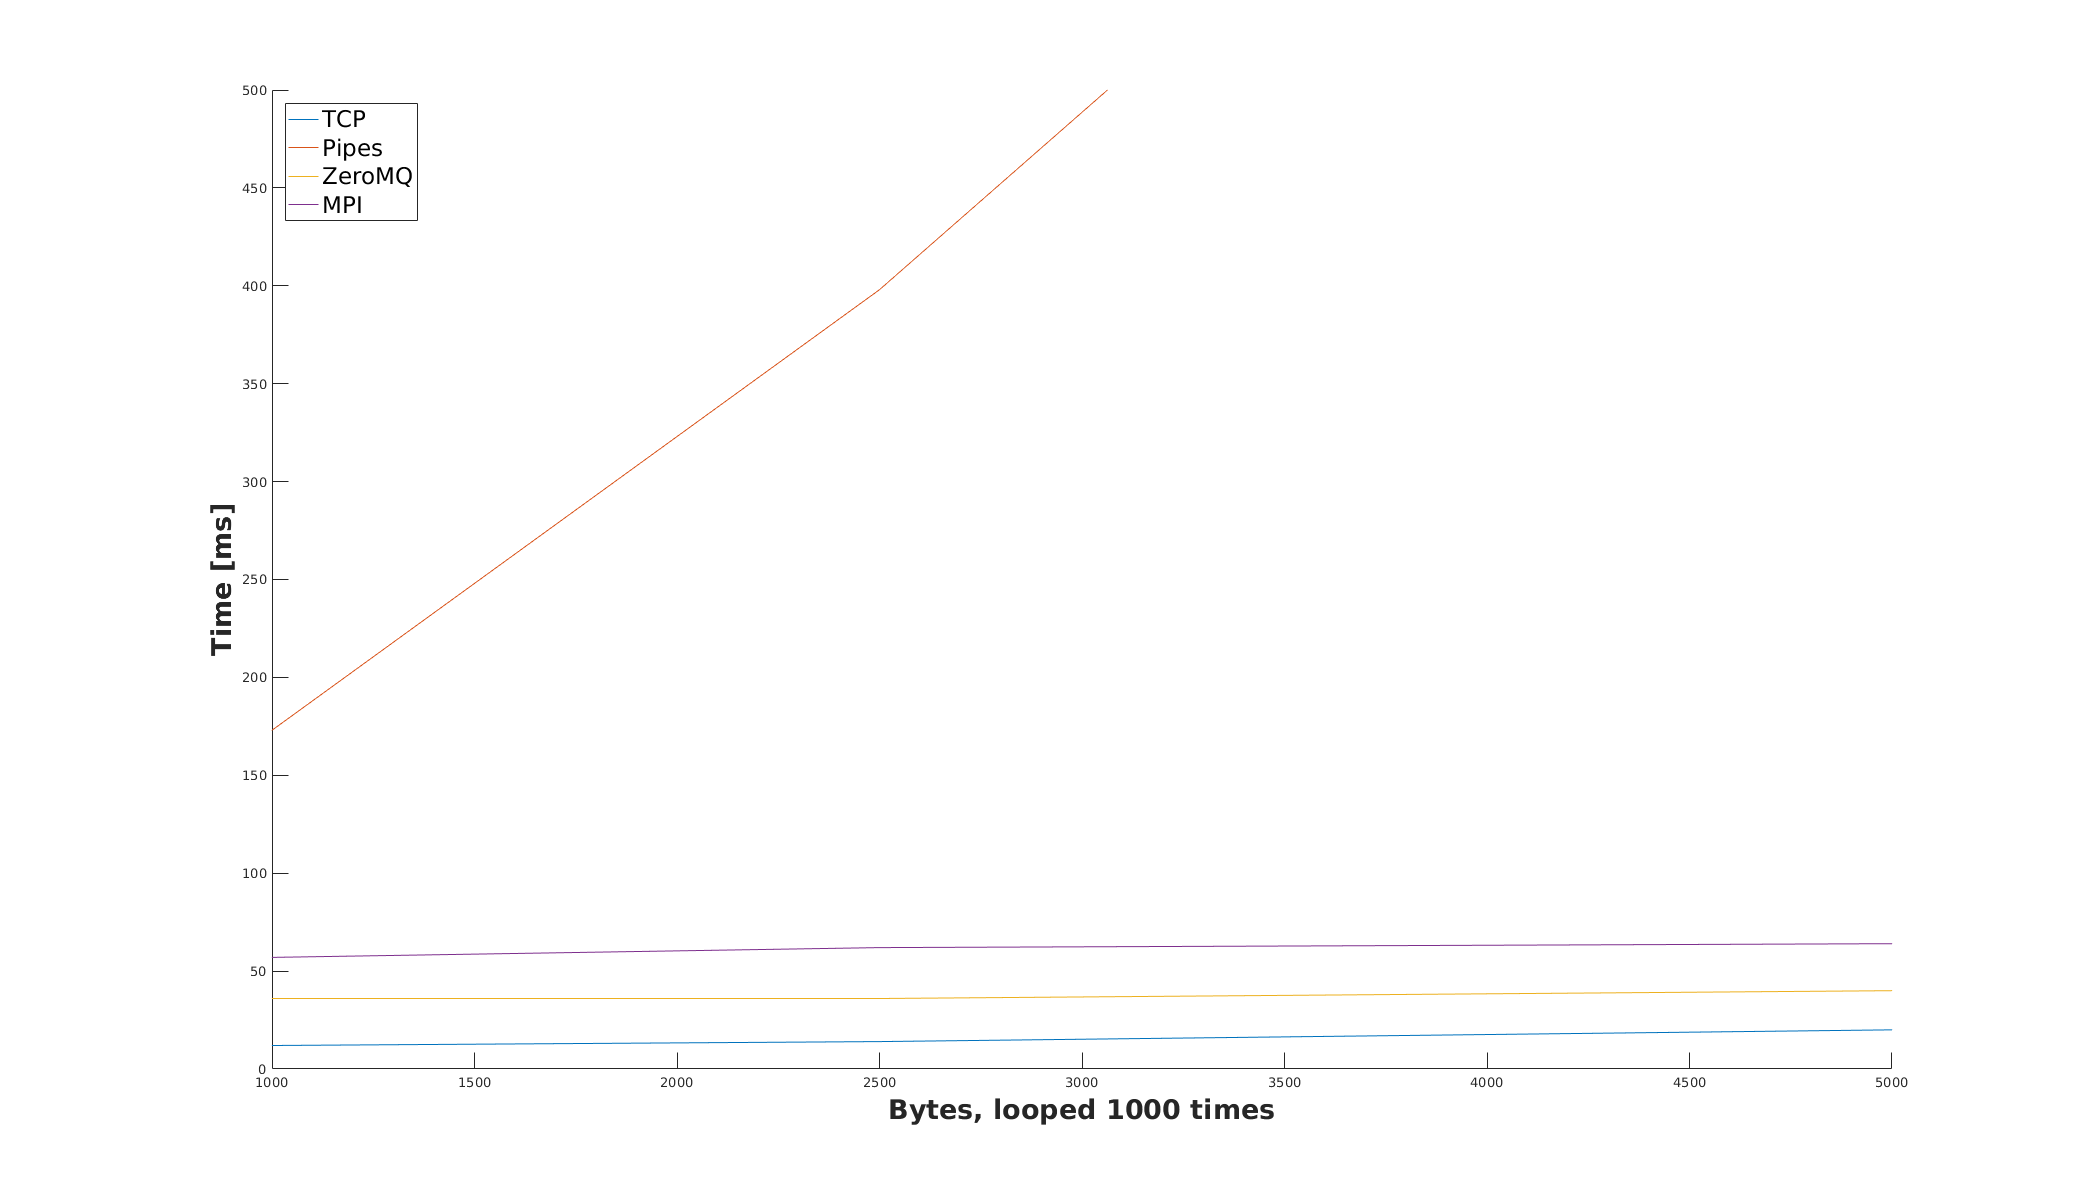
\includegraphics[width=1\columnwidth]{thousandrun-nf}
    \end{figure}
    \end{frame}
%%
    \begin{frame}{Result for I/O Performance}
    \begin{itemize}[<+-|alert@+>]
        \item TCP was the fastest, but the most difficult to implement.
        \item Since we assumed a lot of data would be passed we opted for ZeroMQ
              due to its presumptive ease of use and performance.
    \end{itemize}
    \end{frame}

%%%%%%%%%%%%%%%%%%%%%%%%%%%%%%%%%%%%%%%%%%%%%%%%%%%%%%%%%%%%%%%%%%%%%%%%%%%%%%%

    \section{Implementation}

    \begin{frame}{Implementation}
    \begin{itemize}[<+-|alert@+>]
        \item Installation of ZeroMQ on \bf{bootes}
        \item Porting our code to a different compiler: gfortran $\rightarrow$ ifort
        \item Understanding where to put what and why
        \item A lot of coding
    \end{itemize}
    \end{frame}
%%
    \begin{frame}{Implementation}
        \begin{figure}[h!]
        \centering
        \begin{minipage}{.5\columnwidth}
            \begin{itemize}[<+-|alert@+>]
                \item Two programs:
                \begin{itemize}[<+-|alert@+>]
                    \item child\_com.f
                    \item parent\_com.f
                \end{itemize}
                \item Strategy:
                \begin{itemize}[<+-|alert@+>]
                    \item Open and close the connection as few times as
                          possible
                    \item Send as much data as possible each time
                \end{itemize}
            \end{itemize}
        \end{minipage}%
        \begin{minipage}{.5\columnwidth}
            \centering
            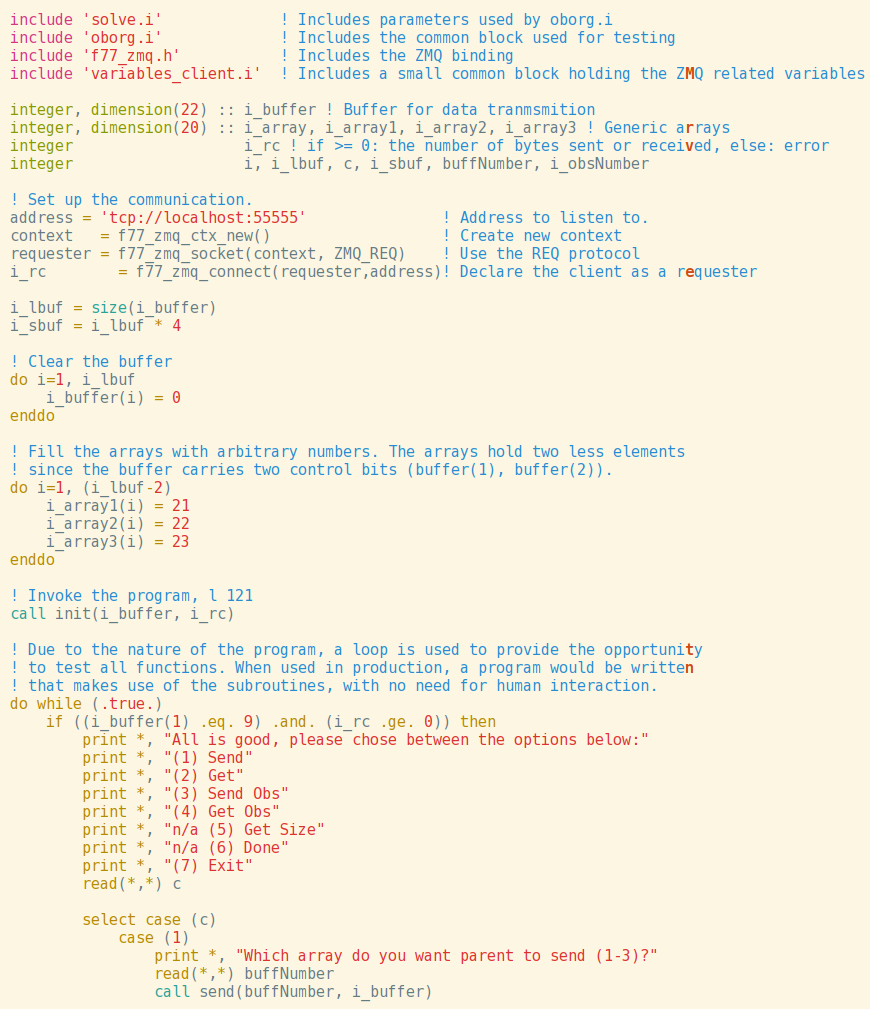
\includegraphics[width=1\columnwidth]{child_com}
        \end{minipage}
        \end{figure}
    \end{frame}


%%%%%%%%%%%%%%%%%%%%%%%%%%%%%%%%%%%%%%%%%%%%%%%%%%%%%%%%%%%%%%%%%%%%%%%%%%%%%%%

    \section{Results for Project One}

    \begin{frame}{Results for Project One}
        Running userpartials for $\sim$200 sessions.
        \pause
        \begin{itemize}[<+-|alert@+>]
            \item Old version of globl/solve: 8 minutes 47 seconds
            \item New version of globl/solve: 9 minutes 5 seconds
        \end{itemize}
    \end{frame}
%%
     \begin{frame}{Results for Project One}
        Running userpartials for $\sim$1400 sessions.
        \pause
        \begin{itemize}[<+-|alert@+>]
            \item Old version of globl/solve: 42 minutes 20 seconds
            \item New version of globl/solve: 46 minutes 34 seconds
        \end{itemize}
    \end{frame}
%%
   \begin{frame}{Results for Project One}
        \centering{Why?}
    \end{frame}
%%
    \begin{frame}{Results for Project One}
        Globl/solve does not \emph{read and write} a lot, it \bf{reads} a lot,
        \centering
        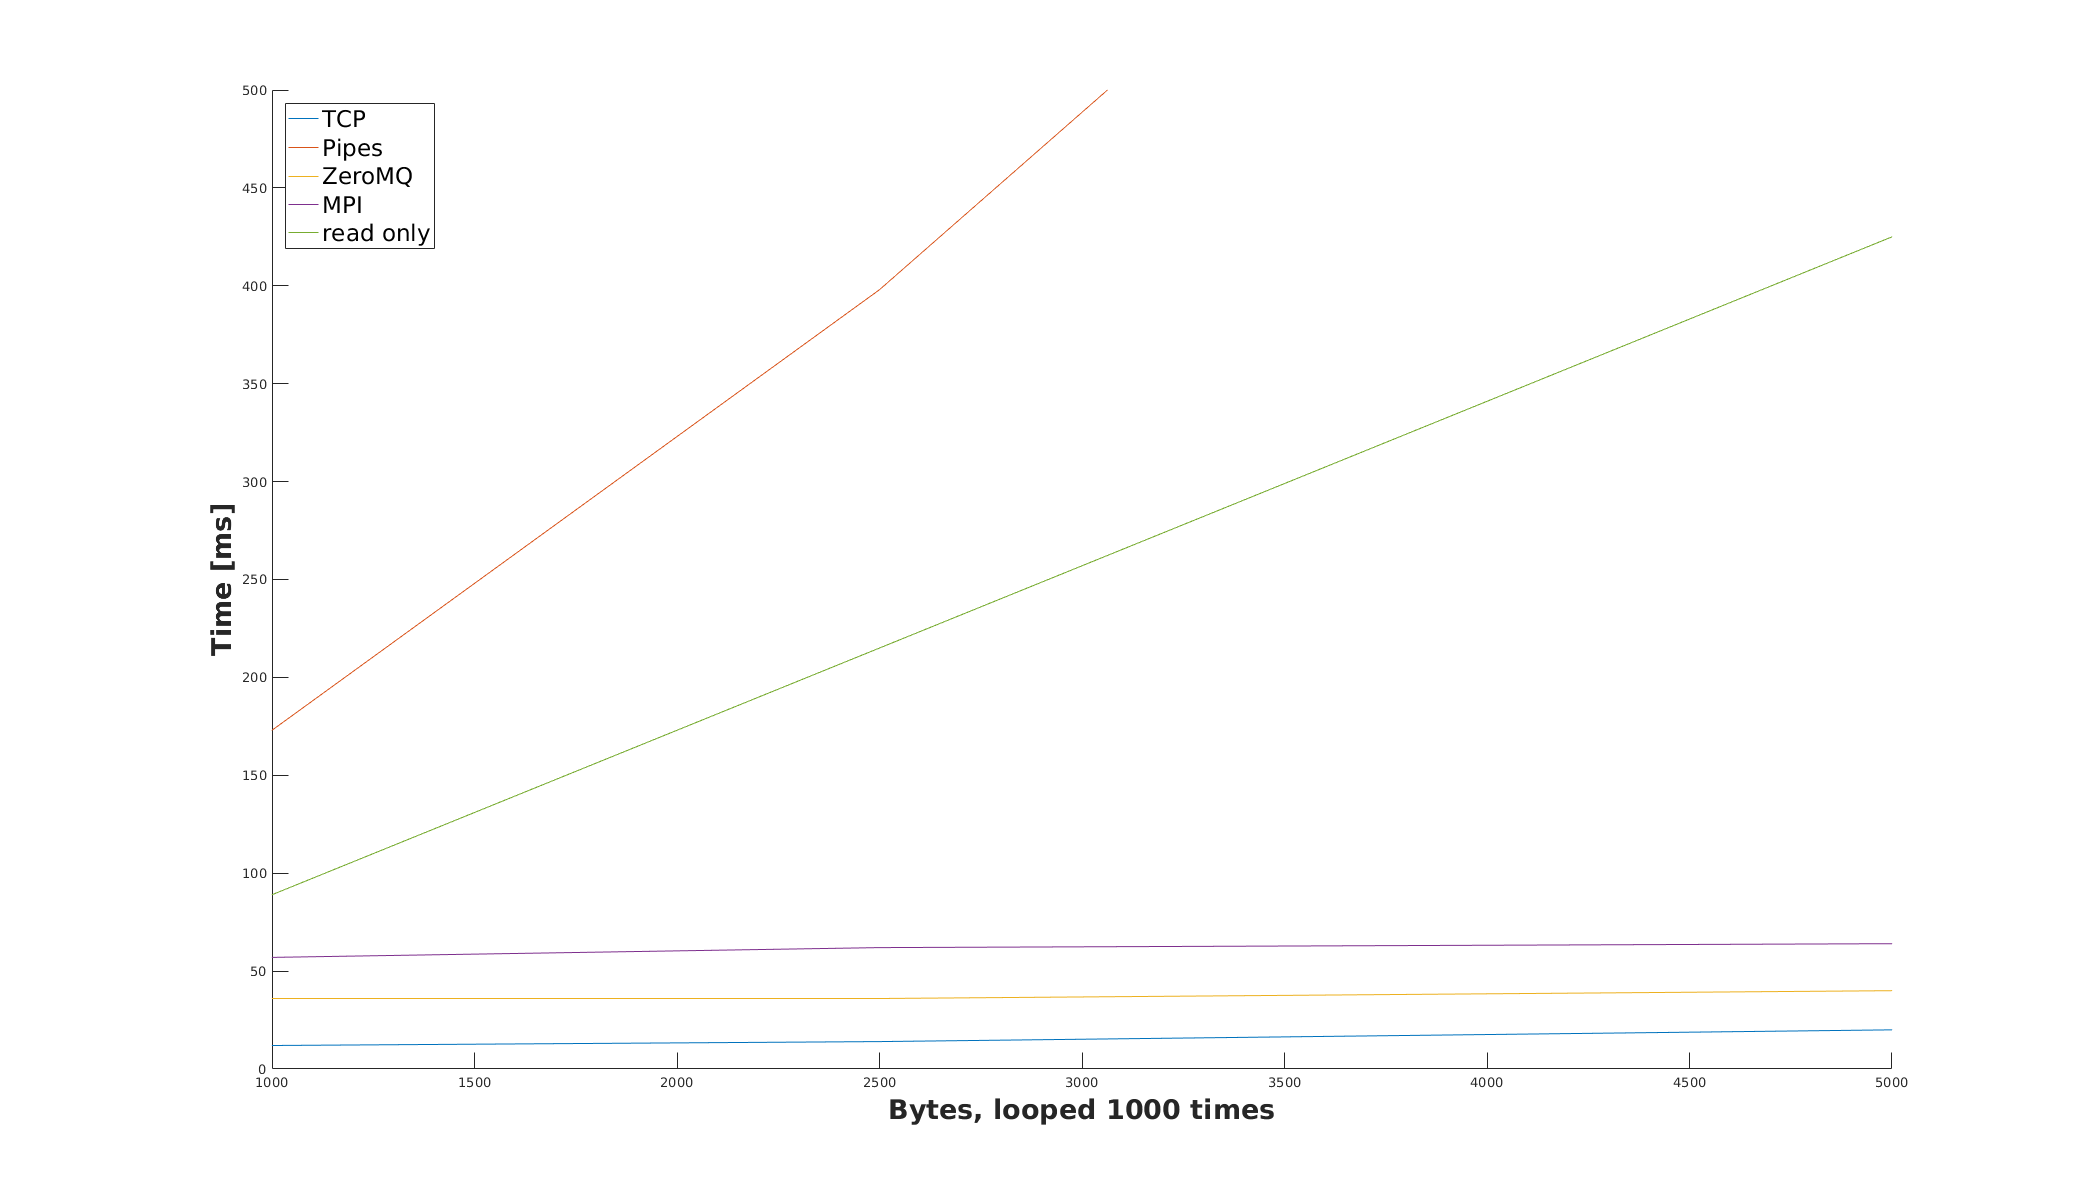
\includegraphics[width=1\columnwidth]{thousandrun}

        but read only is still slower...
    \end{frame}
%%
    \begin{frame}{Results for Project One}
        Globl/solve does not read as much as we thought.
        \centering
        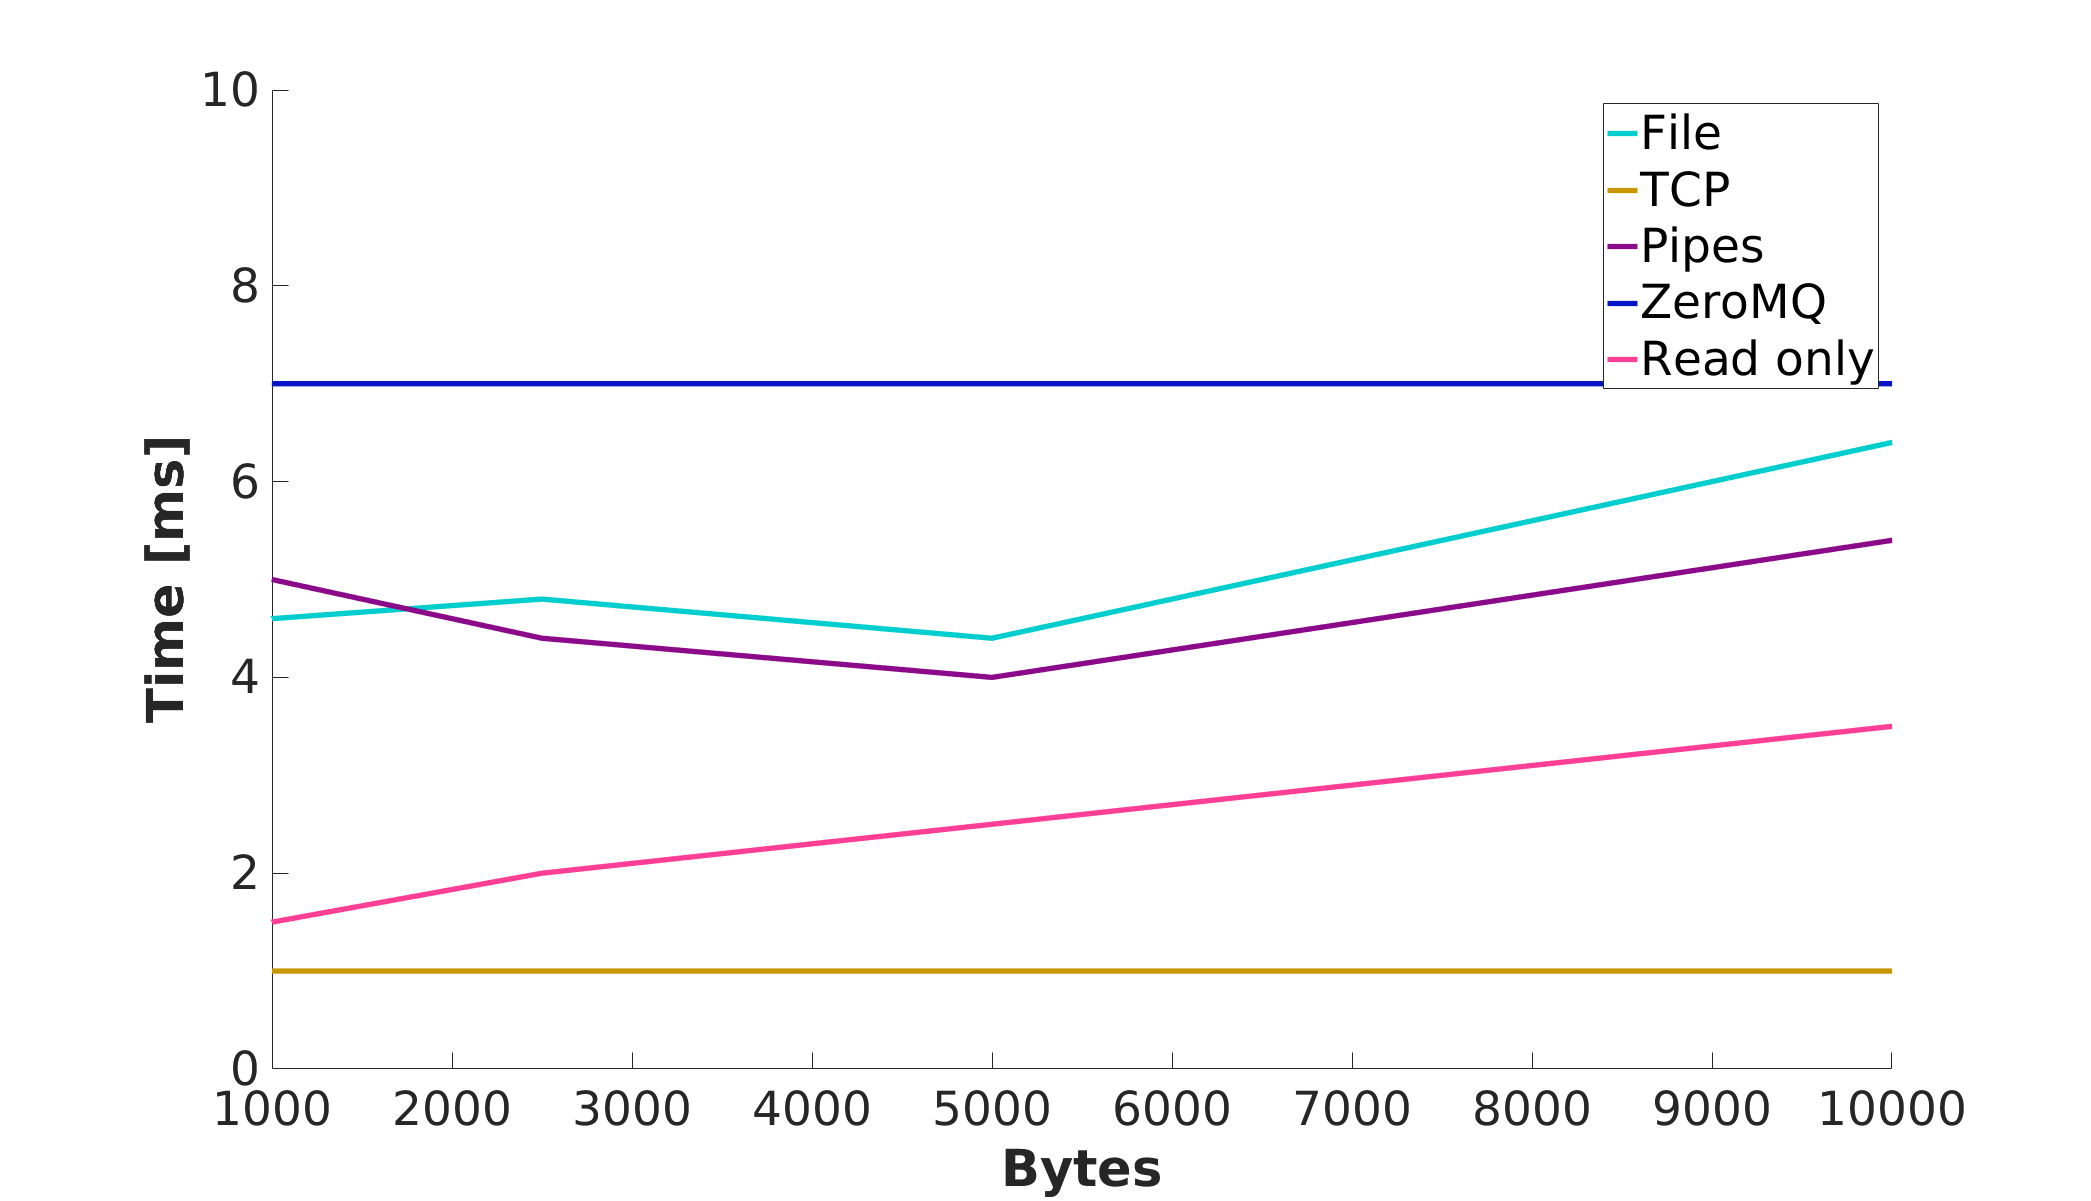
\includegraphics[width=1\columnwidth]{singlerun}
    \end{frame}
%%
    \begin{frame}{Results for Project One}
        Maybe not all in vain:
        \pause
        \begin{itemize}[<+-|alert@+>]
            \item ZeroMQ can be used for concurrency (parallel programming)
            \item We only calculate user partials, what about user programs?
        \end{itemize}
    \end{frame}
%%
    \begin{frame}{Future studies}
        \begin{itemize}[<+-|alert@+>]
            \item Remove the writes that are no longer needed.
            \item TCP should have been the way to go?
            \item Posix Shared Memory?
            \begin{itemize}[<+-|alert@+>]
                \item Conversion between C and Fortran was non trivial.
            \end{itemize}
        \end{itemize}
    \end{frame}

%%%%%%%%%%%%%%%%%%%%%%%%%%%%%%%%%%%%%%%%%%%%%%%%%%%%%%%%%%%%%%%%%%%%%%%%%%%%%%%

    \section{Our Second Project}

    \begin{frame}{Problem Description}
%        Mario noticed that we were getting error msgs about antennas arriving
%        late on source.

        The model used for determining when an antenna acquires a source is a
        little bit off. Sked will say that an antenna should be on target at
        time $T$ but the logfiles tells us that the antenna actually was on
        source at $T \pm c$.
    \end{frame}
%%
    \begin{frame}{Extract the Data}
        \centering
        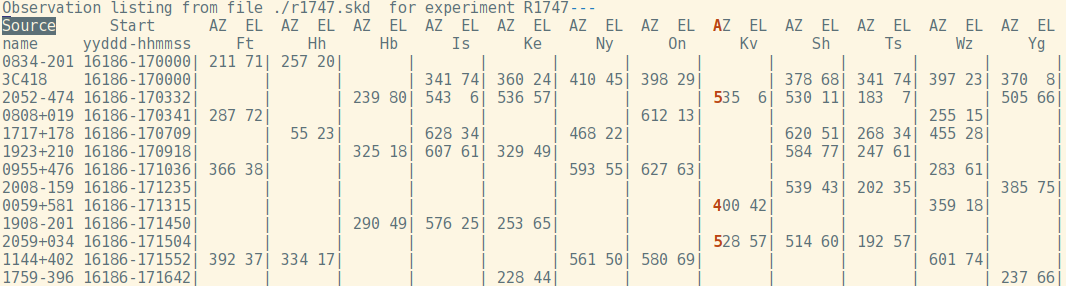
\includegraphics[width=1\columnwidth]{skds}\\[2ex]
        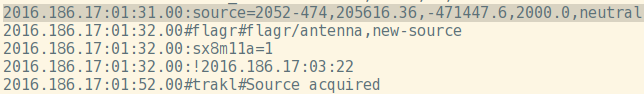
\includegraphics[width=0.75\columnwidth]{logs}
    \end{frame}
%%
    \begin{frame}{Parse the Data}
        \begin{itemize}[<+-|alert@+>]
            \item Correlate the log data with the Sked data.
            \item Least Square Fit
        \end{itemize}
    \end{frame}

%%%%%%%%%%%%%%%%%%%%%%%%%%%%%%%%%%%%%%%%%%%%%%%%%%%%%%%%%%%%%%%%%%%%%%%%%%%%%%%

    \section{Result for Project Two}

%   lista över r17 och stationer


    \begin{frame}{Sessions and stations}
    
        \begin{columns}[T] % align columns
            \begin{column}{.48\textwidth}
            \color{black}\rule{\linewidth}{4pt}

                Sessions used:

                \begin{itemize}
                    \item Regular Monday sessions
                    \begin{itemize}
                        \item r1721 - r1752 
                    \end{itemize}
                    \item Regular Thursday sessions
                    \begin{itemize}
                        \item r4721 - r4752 
                    \end{itemize}
                \end{itemize}

            \end{column}
            \hfill
            \begin{column}{.5\textwidth}
                \rule{\linewidth}{4pt}
                Stations in sessions:
                \begin{columns}[T] % align columns
                    \begin{column}{.5\textwidth}
                        \begin{itemize}
                            \item Badary
                            \item Fortleza
                            \item Hart15m
                            \item Hobart12
                            \item Ishioka
                            \item Kashim34
                            \item Kath12m
                            \item Kokee
                            \item Matera
                            \item Medicina
                            \item Nyales20
                       \end{itemize}
                    \end{column}
                    \begin{column}{.5\textwidth}
                        \begin{itemize}
                            \item Onsala60
                            \item Raegyeb
                            \item Sejong
                            \item Seshan25
                            \item Svetloe
                            \item Tsukub32
                            \item Urumqi
                            \item Yarra12m
                            \item Yebes40m
                            \item Zelenchk
                       \end{itemize}
                    \end{column}
                \end{columns}
            \end{column}%
        \end{columns}
    \end{frame}
%%
    \begin{frame}{Extracted data points}
        \centering
        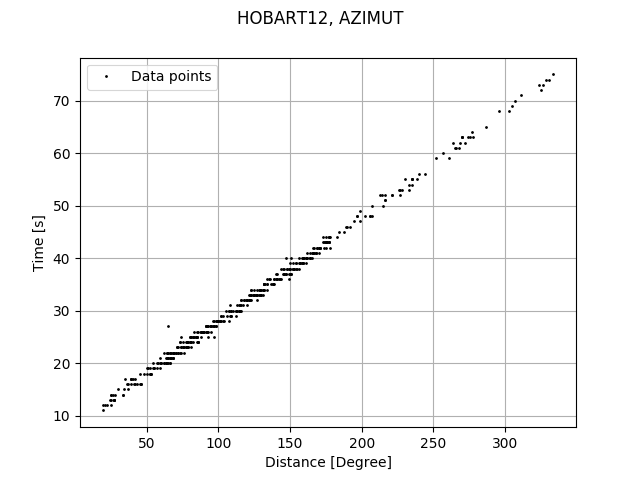
\includegraphics[width=1\columnwidth]{HOBART12_AZIMUT_DATA}
    \end{frame}
%%
    \begin{frame}{Calculated model}
        \centering
        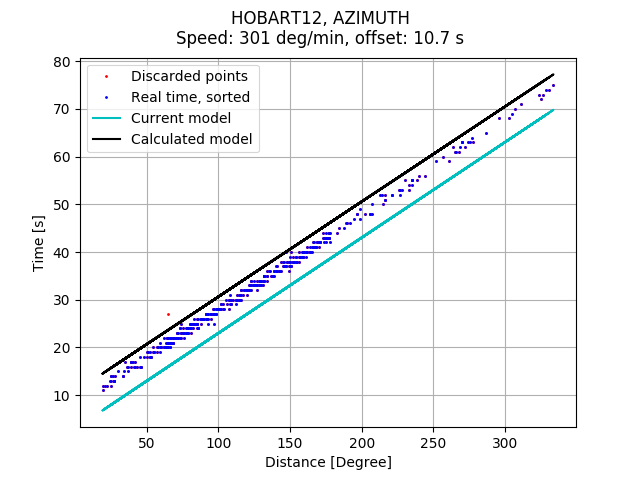
\includegraphics[width=1\columnwidth]{HOBART12_AZIMUT}
    \end{frame}
%%
%% One frame containing AZ info: Old model | New model | Delta
%% One frame containing EZ info: Old model | New model | Delta
%% Talk about how it hasnt been an issue that e.g. Ishioka is "bad", since it's
%a lot faster than the other ones anyway.
    \begin{frame}{Result for Project two}
        \tabcolsep=0.15cm
        \begin{tabular}{l | c c | c c |c c}
            Antenna & $\text{Az}_{\text{Old}}$ & Offset & $\text{Az}_{\text{New}}$ & Offset & $\Delta$Azimuth & $\Delta$Offset \\ [-8pt]
                    & \tiny{[deg/min]}& \tiny{[s]}&\tiny{[deg/min]}&\tiny{[s]}&\tiny{[deg/min]}& \tiny{[s]} \\ 
            \hline
            Badary            & 60  & 40.0  & 65  & 40.2 &  +5 &  +.2 \\
            Fortleza          & 40  &  0.0  & 48  & 16.2 &  +8 &+16.2 \\
            Hart15m           & 120 &  3.0  & 124 & 10.5 &  +4 & +7.5 \\
            Hobart12          & 300 &  3.0  & 301 & 10.9 &  +1 & +7.9 \\
            Ishioka           & 720 & 10.0  & 728 &  9.5 &  +8 &  -.5 \\
            Kashim34          & 45  &  0.0  & 49  & 13.8 &  +4 &+13.8 \\
            Kath12m           & 300 &  3.0  & 300 & 11.0 &   0 &+11.0 \\
            Kokee             & 117 & 15.0  & 127 & 13.4 & +10 & -1.6 \\
            Matera            & 90  & 20.0  & 105 & 37.3 & +15 &+17.3 \\
            Medicina          &  48 &  0.0  & 48  & 13.7 &   0 &+13.7 \\
            Nyales20          & 120 &  9.0  & 137 &  8.2 & +27 & +8.2 \\
        \end{tabular}
    \end{frame}
%%
    \begin{frame}{Result for Project two}
        \tabcolsep=0.15cm
        \begin{tabular}{l | c c | c c | c c}
            Antenna & $\text{Az}_{\text{Old}}$ & Offset & $\text{Az}_{\text{New}}$ & Offset & $\Delta$Azimuth & $\Delta$Offset \\ [-8pt]
                    & \tiny{[deg/min]}& \tiny{[s]}&\tiny{[deg/min]}&\tiny{[s]}&\tiny{[deg/min]}& \tiny{[s]} \\
            \hline
            Onsala60          & 144 &  20 & 184 & 19.0 & +40 & -1.0 \\
            Raegyeb           & 720 &   3 & 718 & 12.8 &  -2 & +9.8 \\
            Sejong            & 300 &   0 & 312 & 22.7 & +12 &+22.7 \\
            Seshan25          &  60 &   0 &  56 & 10.1 &  -4 &+10.1 \\
            Svetloe           &  60 &  40 &  67 & 34.9 & +20 & -5.1 \\
            Tsukub32          & 180 &  14 & 195 & 15.6 & +15 & +1.6 \\
            Urumqi            &  60 &   0 &  61 & 11.3 &  +1 &+11.3 \\
            Yarra12m          &  & &  &  &  \\
            Yebes40m          &  & &  &  &  \\
            Zelenchk          &  & &  &  & \\
        \end{tabular}
    \end{frame}
%%
    \begin{frame}{Mirrored data points}
        \begin{itemize}[<+-|alert@+>]
            \item Some stations has a line of additional data points mirrored
                  in the 180 degree line.
            \item Probably due to cable wrap.
            \item Stations: Ishioka, Kath12m, Sejong and Yarra12m
        \end{itemize}
    \end{frame}
%%
    \begin{frame}{Extracted data points}
        \centering
        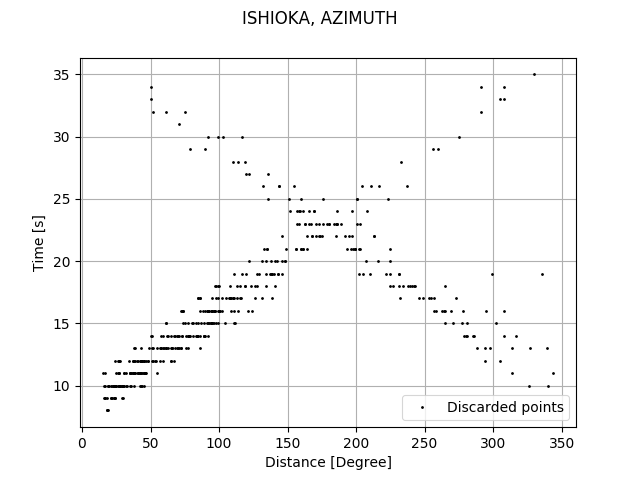
\includegraphics[width=1\columnwidth]{ISHIOKA_AZIMUT_DATA}
    \end{frame}
%%
    \begin{frame}{Calculated model}
        \centering
        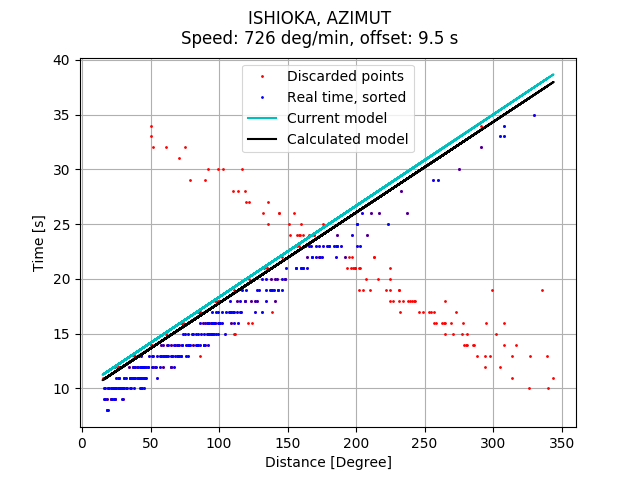
\includegraphics[width=1\columnwidth]{ISHIOKA_AZIMUT}
    \end{frame}

%%
    \begin{frame}{Iteration of Least Square Fit}

    %% Add antenna that does not behave well with the curr thrsh.
    %% Add example where Skd and ours differ a lot!

        \begin{figure}[htp] % not h only
        \centering
        \subfigure{%
            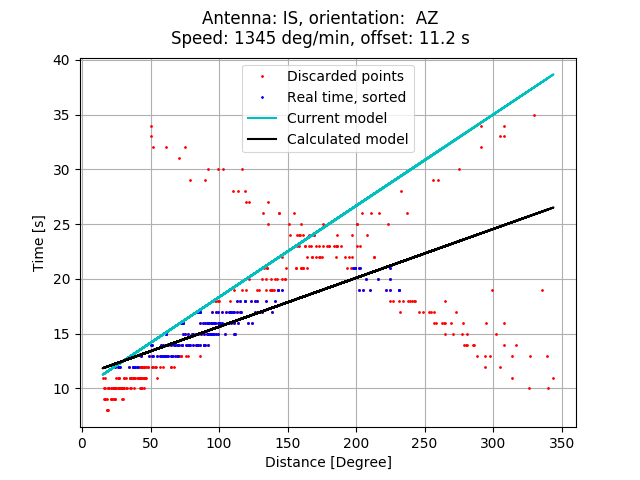
\includegraphics[width=0.4\textwidth]{is_az_1}%
        }\hfil
        \subfigure{%
            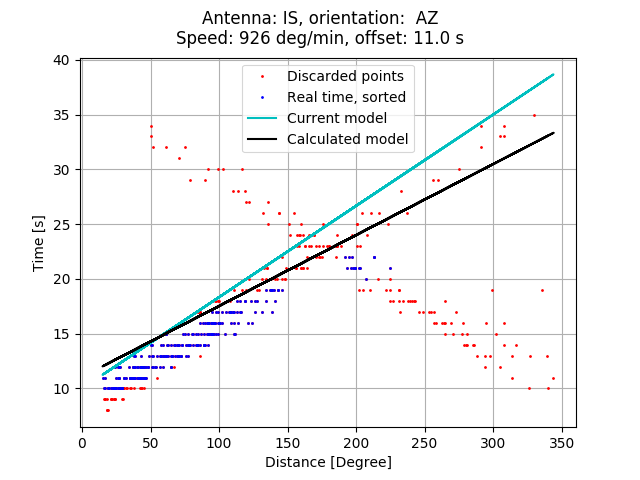
\includegraphics[width=0.4\textwidth]{is_az_3}%
        }

        \subfigure{%
            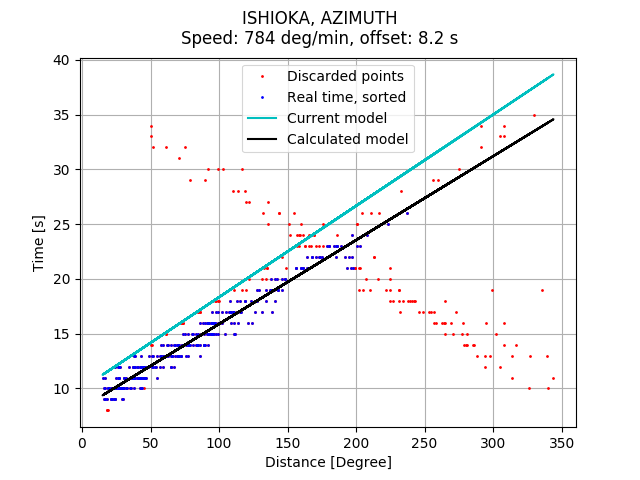
\includegraphics[width=0.4\textwidth]{is_az_5}%
        }\hfil
        \subfigure{%
            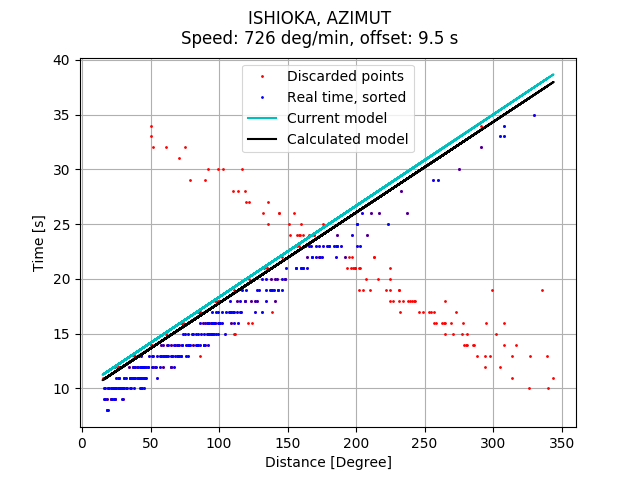
\includegraphics[width=0.4\textwidth]{ISHIOKA_AZIMUT}%
        }
%        \caption{Q metric plotted against time}
        \end{figure}
    \end{frame}
%%
    \begin{frame}{Future studies}
        \begin{itemize}[<+-|alert@+>]
            \item Fix the bug in Sked.
            \item Set a more intelligent threshold.
        \end{itemize}
    \end{frame}
%%
    \begin{frame}
        \centering
%        \includegraphics[width=1\columnwidth]{ENTER}
    \end{frame}
%%
    \begin{frame}{Questions?}
        \centering
        Questions?
    \end{frame}


%%%%%%%%%%%%%%%%%%%%%%%%%%%%%%%%%%%%%%%%%%%%%%%%%%%%%%%%%%%%%%%%%%%%%%%%%%%%%%%

%    \section{Returning Home}
%
%    \begin{frame}{Returning Home}
%        During our time here we have:
%        \pause
%        \begin{itemize}[<+-|alert@+>]
%            \item been exposed to how it is to work at NASA and NVI.
%            \item learned the importance of conducting thorough research.
%            \item realized that patience really is a virtue...
%        \end{itemize}
%    \end{frame}
%
%    \begin{frame}{Returning Home}
%        \centering
%        Thank you! \\ [2ex]
%        \includegraphics[width=1\columnwidth]{interns}
%    \end{frame}
%
\end{document}

